\newcommand{\gscale}{2}
\begin{figure*}
\centering
\subfigure[Original Gadget]{
	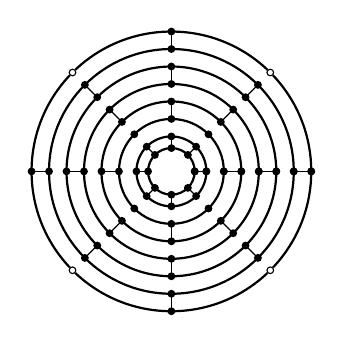
\begin{tikzpicture}[scale=\gscale,cap=round]
	%all cycles
	\foreach \r in {.148,.222,.333,.444,.555,.666,.777,.888}{
		\draw[thick] (0cm,0cm) circle(\r cm);
	}
	%all nodes but the outermost
	\foreach \r in {.148,.222,.333,.444,.555,.666,.777}{
		 \foreach \x in {0,45,...,360} {
			\filldraw[black] (\x:\r cm) circle(0.6pt);
		}
	}
	\foreach \x in {0,90,...,360} {
		\filldraw[black] (\x:.888 cm) circle(0.6pt);
	}
	\foreach \x in {45,135,...,360} {
		\filldraw[white] (\x:.888 cm) circle(0.6pt);
		\draw[black] (\x:.888 cm) circle(0.6pt);
	}

	%draw edges
	\foreach \x in {0,90,...,360} {
	 	\filldraw[black] (\x:.777) -- (\x:.888);
	 	\filldraw[black] (\x:.555) -- (\x:.666);
	 	\filldraw[black] (\x:.333) -- (\x:.444);
	 	\filldraw[black] (\x:.148) -- (\x:.222);
	}
	%draw other edges
	 \foreach \x in {45,135,...,360} {
	 	\filldraw[black] (\x:.666) -- (\x:.777);
	 	\filldraw[black] (\x:.444) -- (\x:.555);
	 	\filldraw[black] (\x:.148) -- (\x:.222);
	} 
	\end{tikzpicture}
	\label{fig:orig-gadget}
}
\subfigure[Modified Gadget]{
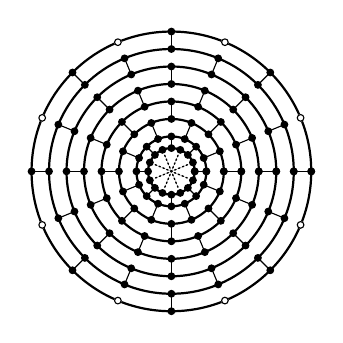
\begin{tikzpicture}[scale=\gscale,cap=round]
% draw the nested circlesn{tikzpicture}[scale=5.3,cap=round,>=latex]
% draw the unit circle

%all circles
\foreach \r in {.148,.222,.333,.444,.555,.666,.777,.888}{
	\draw[thick] (0cm,0cm) circle(\r cm);
}

%all nodes but the outermost radius
\foreach \r in {.148,.222,.333,.444,.555,.666,.777}{
	 \foreach \x in {0,225,...,3600} {
		\filldraw[black] (\x/10 : \r cm) circle(0.6pt);
	}
}
%outermost degree three
\foreach \x in {0,450,...,3600} {
	\filldraw[black] (\x/10 : .888 cm) circle(0.6pt);
}

%outermost outlet nodes
\foreach \x in {225,675,...,3600} {
	\filldraw[white] (\x/10 : .888 cm) circle(0.6pt);
	\draw[black] (\x/10 : .888 cm) circle(0.6pt);
}


%draw edges
\foreach \x in {0,450,...,3600} {
	\filldraw[black] (\x/10:.777) -- (\x/10:.888);
	\filldraw[black] (\x/10:.555) -- (\x/10:.666);
	\filldraw[black] (\x/10:.333) -- (\x/10:.444);
	\filldraw[black] (\x/10:.148) -- (\x/10:.222);
}

%fill in the interior cycle     
\filldraw[densely dotted, line width=.5pt] (225/10:.111) -- (2025/10:.111);
\filldraw[densely dotted, line width=.5pt] (675/10:.111) -- (2475/10:.111);
\filldraw[densely dotted, line width=.5pt] (1125/10:.111) -- (2925/10:.111);
\filldraw[densely dotted, line width=.5pt] (1575/10:.111) -- (3375/10:.111);

%draw other edges
\foreach \x in {225,675,...,3600} {
 	\filldraw[black] (\x/10:.666) -- (\x/10:.777);
 	\filldraw[black] (\x/10:.444) -- (\x/10:.555);
 	\filldraw[black] (\x/10:.333) -- (\x/10:.222);
}   
\label{fig:mod-gadget}
\end{tikzpicture}
}
\caption{Each local replacement gadget replaces vertices in the 
	 original graph so edges originally incident to a vertex are attached to
	 vertices on the outermost cycle. We modify the original 
	 construction so that this operation produces a 3-regular graph, instead
	 of a degree at most three graph. To do this use the new gadget and then simply pair off remaining vertices on the outermost layer
	 possibly adding a few vertices to make all gadgets have an equal number of pairs.}
\label{fig:gadgets}
\end{figure*}
